
\begin{frame}
\frametitle{Conception d'un schéma}

\alert{Cassandra ne propose pas de jointure}. C'est du NoSQL après tout.

\vfill

Il est donc préférable de \alert{regrouper} les données le plus possible dans des lignes
(notion de document autonome, déjà vue).

\vfill


Au pire, on peut représenter les mêmes données sous plusieurs formes.

\begin{redbullet}
  \item Tous les patients, avec leurs pathologies.
  \item Toutes les pathologies, avec les occurrences de cas
\end{redbullet}


\vfill

Le regroupement a aussi des inconvénients (redondance, difficulté d'accès aux
données ``profondes''). 
\end{frame}


\begin{frame}[fragile]
\frametitle{Imbrication de structures}

C'est le principe de dénormalisation\,: on regroupe 
les données le plus possible dans des lignes pour éviter les jointures.

\vfill

Une valeur d'attribut  peut correspondre\,:
\begin{redbullet}
	\item à un ensemble de valeurs (non ordonnées)\,: \textbf{SET} 
	\item à une liste de valeurs\,: \textbf{LIST}
	\item à un dictionnaire (objet)\,: \textbf{MAP} 
	\item à une instance d'un type utilisateur
\end{redbullet}

\vfill

Les ensembles doivent rester de taille raisonnable
\end{frame}


\begin{frame} \frametitle{Le langage CQL}

Cassandra propose un langage, nommé CQL, inspiré de SQL, 
mais fortement restreint par l'absence de jointure. 

\vfill

CQL ne permet d'interroger qu'une seule table\,!

\vfill

De plus, d'autres types de restrictions s'appliquent\,! Elles s'expliquent toutes
par la volumétrie potentielle des tables.

\vfill

Nous allons étudier
tout cela.
\end{frame}



\begin{frame}[fragile] \frametitle{Premiers pas}

Sélectionnons tous les départements.

\begin{minted}{sql}
select  * from departement;
\end{minted}

\vfill

Ou seulement les 20 premiers.
\begin{minted}{sql}
select  * from departement limit 20;
\end{minted}

\vfill
Retour en JSON
\begin{minted}{sql}
select JSON * from departement;
\end{minted}

\vfill
Accédons à un objet imbriqué.
\begin{minted}{sql}
select nom, region.nom from departement;
\end{minted}

\vfill
En revanche, on ne peut pas accéder aux éléments d'un ensemble.
\begin{minted}{sql}
select nom, departements.nom from region;
\end{minted}
\end{frame}

\begin{frame}[fragile] \frametitle{La clause \texttt{where}}

Sélectionnons un film.

\begin{minted}{sql}
select  *  from region where id='iuv';
\end{minted}

Ou plusieurs

\begin{minted}{sql}
select  * from region 
    where id in ('iuv', 'r44', 'x45');
\end{minted}
 
Et si ce n'est pas la clé\,?

\begin{minted}{sql}
select  * from departement where nom='Loire' ;
\end{minted}

\begin{verbatim}
Unable to execute CQL script. Cannot execute this query 
as it might involve data
filtering and thus may have unpredictable performance. 
\end{verbatim}

Essayons de comprendre.
\end{frame}

\begin{frame}[fragile] \frametitle{Structure d'un schéma}

\begin{columns}
    \begin{column}{0.45\textwidth}
  
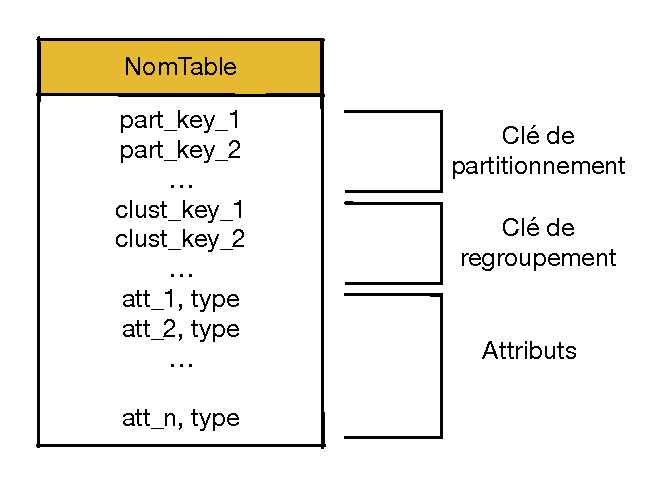
\includegraphics[height=.8\textwidth]{../figures/cassandra_chebotko_fr.pdf}
  \end{column}
 \begin{column}{0.45\textwidth}
 \begin{minted}{sql}
 create table Tname (
   part_key_1 type,
   part_key_2 type,
   ... type,
   clust_key_1 type,
   ... type,
   att_1 type,
   att_2 type,
   ... type,
   primary key ( 
       (part_key_1, part_key2, ...), 
       (clust_key_1, clust_key_2, ...) 
       )
 )
 \end{minted}
\end{column}
\end{columns}

\end{frame}



\begin{frame}[fragile] \frametitle{Exemple\,: organisons régions et départements}

\begin{minted}{sql}
    create table Departement (
        id_region int,
        id_departement int,
        nom text,
        primary key (id_region, id_departement)
     ) 
\end{minted}
\vfill

\begin{redbullet}
  \item La clé de partitionnement est  l'identifiant de la région
  \item La clé de regroupement est l'identifiant du département
\end{redbullet}
\end{frame}


\begin{frame}[fragile] \frametitle{Clé de partitionnement = placement}

\begin{columns}
    \begin{column}{0.45\textwidth}
  
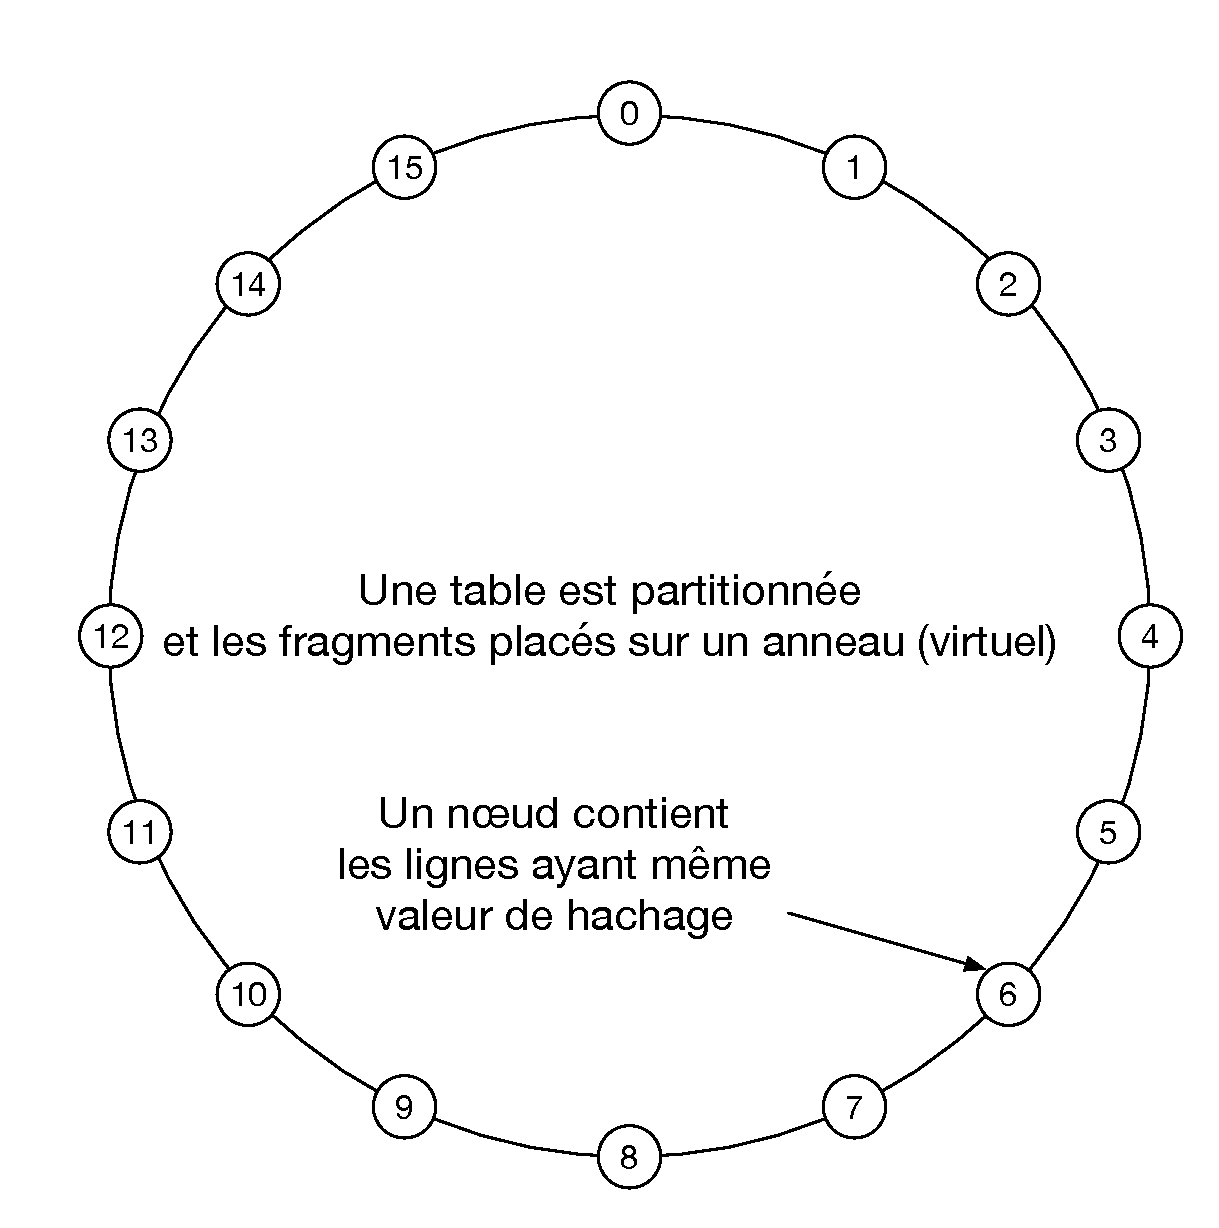
\includegraphics[height=\textwidth]{../figures/cassandra_anneau.pdf}
  \end{column}
 \begin{column}{0.45\textwidth}
\begin{redbullet}
		\item Pour chaque ligne on applique une fonction de hachage 
		          aux valeurs de la clé de \alert{partitionnement}
		\item La valeur de hachage détermine le placement dans le système distribué
		\item $\Rightarrow$ une requête incluant comme critère une clé de partitionnement
		     ne concerne qu'un seul serveur
	\end{redbullet}

\end{column}
\end{columns}

\end{frame}

%%%%%%%%%%
\begin{frame}[fragile] \frametitle{Clé de regroupement = contiguité}

\begin{columns}
    \begin{column}{0.45\textwidth}
    
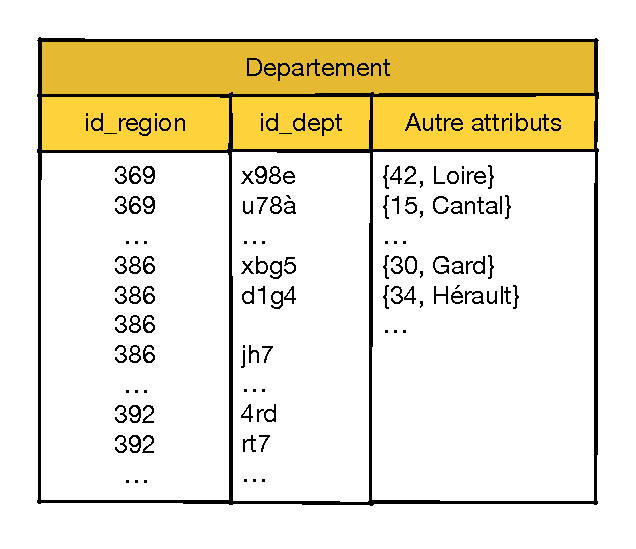
\includegraphics[height=\textwidth]{../figures/cassandra_clustering_fr.pdf}
  
  \end{column}
 \begin{column}{0.45\textwidth}
\begin{redbullet}
		\item Dans un fragment (sur un serveur) les lignes sont triées 
		sur la clé primaire 
		\item Pour une même valeur de partitionnement,  les lignes 
		   sont \alert{consécutives} et ordonnées sur la clé de regroupement
		\item $\Rightarrow$ une requête sur une préfixe de la clé 
		    primaire (part. + regroupement)
		     correspond à un parcours \alert{séquentiel} sur un seul nœud
	\end{redbullet}

\end{column}
\end{columns}

\end{frame}


%%%%%%%%%%
\begin{frame}[fragile] \frametitle{Restrictions sur les requêtes}

Toute recherche sur des critères autres qu'un préfixe de la clé entraîne un parcours
séquentiel

\vfill

Cassandra est conçu pour de très grandes bases de données, et le rejet 
de ces requêtes séquentielles est une précaution. 

\vfill

Principe: Cassandra limite les requêtes à celles dont le coût est proportionnel à la 
taille du résultat.

\vfill

On peut outrepasser avec la clause \texttt{allow filtering}.
\begin{minted}{sql}
select  * from departeme,nt 
     where nom='Loire' allow filtering;
\end{minted}


\end{frame}



\begin{frame}[fragile]
\frametitle{À retenir}

\begin{redbullet}
   \item CQL est un pseudo-sql très limité : pas de jointure ou de capacité
       à interroger les structures imbriquées
   \item Le langage est conçu  pour accéder \alert{efficacement} à de très grosses
      bases, mais avec de très fortes limitations sur les requêtes
   \item Réciproquement, il faut concevoir le schéma pour tirer parti
   de ces principes.
\end{redbullet}
\end{frame}
\end{document}